\documentclass[main.tex]{subfiles}
\begin{document}
\chapter{Quantum chromodynamics in practice}
\label{chapter:qcd}
    In the previous chapter we introduced the basic concepts
    of QCD and setup the framework of calculating
    cross-sections. Cross-sections are the most relevant
    quantities to compute as they can be measured
    experimentally, and are a property of the particles
    being collided, rather than depending on the
    specifics of the experimental procedure.
    This provides a bridge to compare
    theoretical predictions and experiment.
    From (\ref{eqn:dsigma}, the partonic cross-section
    is the matrix element integrated over the relevant
    final-state phase-space, normalised by a flux factor.
    The matrix elements are
    calculated order-by-order in the strong coupling
    $\alpha_{\mathrm{s}}$, (\ref{eqn:matrix_element}),
    where each order corresponds to a set of Feynman diagrams
    that have the appropriate number of vertices,
    as each QCD vertex brings along a factor of $\alpha_{\mathrm{s}}$.

    In this chapter we will discuss the problems that
    arise when evaluating these Feynman diagrams and outline
    some solutions that have been widely adopted to circumvent
    these issues to provide real-world applicable predictions.
    This chapter forms the theoretical foundations on which
    the work of this thesis is built upon.

    We will consider the divergent nature of matrix
    elements and introduce the most widely used techniques
    to tame these singularities.

\section{Divergent structures}
    We have seen that matrix element computations
    result in evaluating Feynman diagrams. From
    the QCD Feynman rules (ref here), it becomes
    clear that integrating over all momentum modes
    will give rise to singularities. The divergences
    associated with high energy modes are ultraviolet
    (UV) divergences. On the opposite end of the energy
    spectrum, low energy modes also give rise to 
    infrared (IR) divergences.

    The de-facto methods to alleviate these
    divergences are through regularisation
    for UV divergences, and through subtraction
    schemes for IR divergences. Both of these
    methods will be discussed in this section.

\subsection{Ultraviolet divergences}
    In loop diagrams we have to evaluate integrals of the form
    \begin{equation}
        \int_{0}^{\Lambda} \dfrac{\mathrm{d}^{4}k}{(2\pi)^{4}}\dfrac{1}{k^{2}(k+p)^{2}} \sim \log{\Lambda} \, ,
    \end{equation}
    where a cutoff scale $\Lambda$ has been introduced to
    capture the divergence as the loop momenta
    $k \rightarrow \infty$. It is clear that the
    integral divergences in this high energy limit,
    hence the name ultraviolet divergence.
\subsection{Renormalisation}
\subsection{Running of the coupling constant}
    The behaviour of $\alpha_{\mathrm{s}}$
    is governed by the Callan-Symanzik \cite{Callan:1970yg,Symanzik:1970rt}
    $\beta$-function
    \begin{equation}\label{eqn:beta_fn}
        \mu^{2} \dfrac{\partial \alpha_{\mathrm{s}}(\mu^{2})}{\partial \mu^{2}} = \beta(\alpha_{\mathrm{s}}) \, ,
    \end{equation}
    where the $\beta$-function can be written as a perturbative
    expansion in $\alpha_{\mathrm{s}}$
    \begin{equation}\label{eqn:beta_series}
        -\beta(\alpha_{\mathrm{s}}) = \sum_{n=0}^{\infty}\dfrac{\alpha_{\mathrm{s}}^{n+2}}{(4\pi)^{n+1}} \beta_{n}\, .
    \end{equation}
    where the coefficients $\beta_{n}$ have been computed
    up to fifth order \cite{Baikov:2016tgj,Luthe:2017ttg}.
    The coefficients computed up to this point have been
    strictly positive, meaning that $\alpha_{\mathrm{s}}$
    decreases with increasing energy due to the minus sign
    in (\ref{eqn:beta_series}), a property known as
    asymptotic freedom \cite{Gross:1973id,Politzer:1973fx}.
    The solution to (\ref{eqn:beta_fn}) to first order
    is
    \begin{equation}\label{eqn:1l_alpha}
        \alpha_{\mathrm{s}}(\mu^{2}) = \dfrac{1}{\frac{\beta_{0}}{4\pi}\log\left(\frac{\mu^{2}}{\Lambda_{\mathrm{QCD}}^{2}}\right)} \, ,
    \end{equation}
    where $\Lambda_{\mathrm{QCD}}$ is the QCD scale,
    the scale at which $\alpha_{\mathrm{s}}$ becomes
    large enough that perturbation theory breaks down.
    The running of the coupling constant has been
    observed experimentally as can be seen in Figure~\ref{fig:alpha_s_running}.
    \begin{figure}
        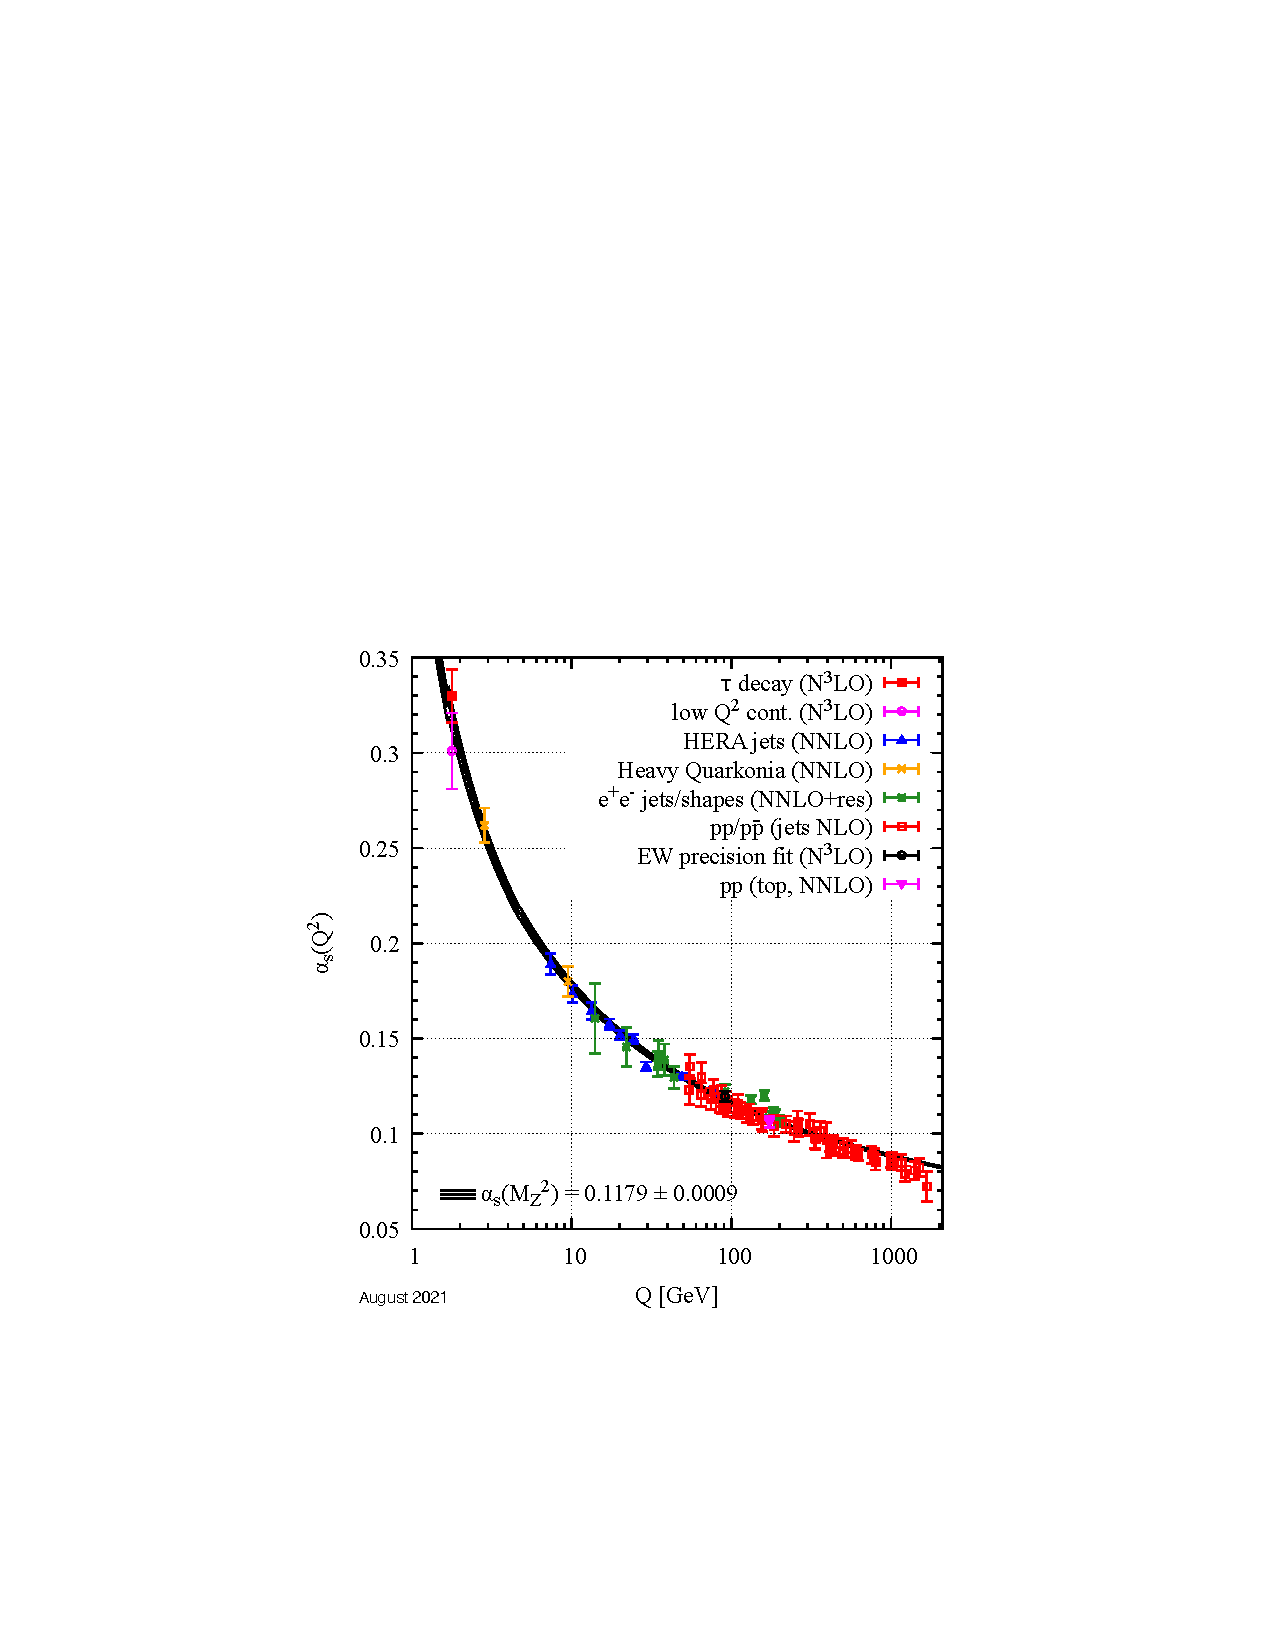
\includegraphics{qcd/alpha_s_running.pdf}
        \caption{The running of the strong coupling constant $\alpha_{\mathrm{s}}$,
        as determined by experiments, with QCD theory prediction in black.
        Figure reference \cite{Workman:2022ynf}.}
        \label{fig:alpha_s_running}
    \end{figure}
    Another consequence of the running coupling
    is colour confinement, in which quarks and
    gluons cannot exist as free particles. Due
    to the increasing strength of coupling at low
    energies, quarks and gluons are forced to
    form composite, colourless particles, known as
    hadrons. The most common example of a hadron
    is the proton which is the origin of the name
    Large Hadron Collider.
\subsection{Infrared divergences}
\subsection{Factorisation of matrix elements}
\subsubsection{Soft limits}
\subsubsection{Collinear limits}

\section{Subtraction}
\subsection{Catani-Seymour dipoles}
\subsection{Antenna subtraction}
\end{document}